%%%%%%%%%%%%%%%%%%%%%%%%%%%%%%%%%%%%%%%%%%%%%%%%%%%%%%%%%%%%%%%%%%%%%%%%%%%%%
%%%                               PLOT2D                                  %%%
%%%%%%%%%%%%%%%%%%%%%%%%%%%%%%%%%%%%%%%%%%%%%%%%%%%%%%%%%%%%%%%%%%%%%%%%%%%%%
\subsubsection{Plot2d}
\label{sec:uiplot2d}
Plots of type \PLOTTWOD{} can be used to produce 2-dimensional graphs of datapool values.
\index{PLOT2D@\PLOTTWOD}
\index{Plot!Plot2d}

\input{diagrams/ui_plot2d_list}
\index{XRTGRAPH@\XRTGRAPH!use \PLOTTWOD}

Pressing the right mouse button within such a diagram pops up a menu which
provides additional configuration functions.
See \nameref{dia:uiplot2dmenuentrylist} on page \pageref{dia:uiplot2dmenuentrylist}.

\paragraph{UI Mode}
\label{par:uiplot2duimode}
\index{PLOT2D@\PLOTTWOD!UI Mode}
\index{PLOT2D\_UIMODE@\PLOTTWODUIMODE!predefined datapool item}
One option in that menu is the UI Mode. The UI Mode defines the behaviour
of the left mouse button inside the plot2ds.

The mode can be changed using
\begin{itemize}
  \item that menu
  \item keyboard shortcuts (when focus is on a \PLOTTWOD)
  \item \DATAPOOL{} variable \PLOTTWODUIMODE
\end{itemize}

The first two ways automatically change the value of \PLOTTWODUIMODE{}.

All \PLOTTWOD{}s within one application share one global UI Mode.
The following modes exist:

\begin{tabularx}{\textwidth}{p{4cm}|X}
UI Mode           & Shortcut (hint) \PLOTTWODUIMODE{} value \newline
                    description \\
\hline
Zoom              &  Ctrl-S (scale) ``ZOOM'' \newline
                     Select a rectangle to zoom in. \\
Select Point      & Ctrl-D (dot) ``SELECT\_POINT'' \newline
                    Select a point (not a line) of a plot curve. \newline
                    If the plot2d has the \FUNC{} option, that function is called
                    and \REASONSELECTPOINT{} is set. \INDEX{} is set to the index
                    of the selected point.
                    The function can access the coordinates of the point using the datapool variables
                    Global\_Point.X and Global\_Point.Y. \newline
                    Without the \FUNC{} option, you can select multiple points.
                    Select the same point again to unselect it. Use \GETSELECTION{} in a function
                    to get the information about the selected points.
                    See \nameref{dia:guimorestatement} on page \pageref{dia:guimorestatement}. \\
Select Rectangle  & Ctrl-A (area) ``SELECT\_RECTANGLE'' \newline
                    This mode is only available when the \FUNC{} option is set.
                    That function is called after selecting a rectangle and \REASONSELECTRECTANGLE{} is set.
                    The function can access the coordinates of the rectangle using the datapool variables
                    Global\_Rect.X1,  Global\_Rect.X2, Global\_Rect.Y1 and Global\_Rect.Y1. \\
\end{tabularx}
\vspace{0.5cm}

\paragraph{Global Symbolsize}
\label{par:uiplot2symbolsize}
\index{PLOT2D@\PLOTTWOD!Global Symbolsize}
\index{PLOT2D\_SYMBOLSIZE@\PLOTTWODSYMBOLSIZE!predefined datapool item}
The symbol sizes of \PLOTTWOD{} curves are normally defined in the resource file.
The user can change them using the option Configuration... in the right mouse button menu of a \PLOTTWOD.

And the symbol size of all \PLOTTWOD{} can be changed to the same value using
the \DATAPOOL{} variable \PLOTTWODSYMBOLSIZE{}. When that variable has a value,
it is used. When the value is cleared, the \PLOTTWOD{}s use the configured symbol sizes again.


\label{uiplot2doptions}
\input{diagrams/ui_plot2d_option}

\index{CAPTION@\CAPTION!plot2d option}
\index{PRINTSTYLE@\PRINTSTYLE!plot2d option}
\index{TRUE@\TRUE!plot2d option printstyle}
\index{HIDDEN@\HIDDEN!plot2d option}
\index{MINMAX@\MINMAX!plot2d option}
\index{RMS@\RMS!plot2d option}
\index{AVG@\AVG!plot2d option}
\index{PLOT2D@\PLOTTWOD!CAPTION@\CAPTION}
\index{PLOT2D@\PLOTTWOD!PRINTSTYLE@\PRINTSTYLE}
\index{PLOT2D@\PLOTTWOD!HIDDEN@\HIDDEN}
\index{PLOT2D@\PLOTTWOD!MINMAX@\MINMAX}
\index{PLOT2D@\PLOTTWOD!RMS@\RMS}
\index{PLOT2D@\PLOTTWOD!AVG@\AVG}
\begin{tabularx}{\textwidth}{l|X}
options     & description \\
\hline
string      & Menutext \\
\CAPTION    & Footertext: Title displayed in the graphics-form. (Using special-characters such as space, you need to use string-representation.) \newline
              identifier may also refere to a previously declared stream. \\
\PRINTSTYLE & = \TRUE{} prints out graph descriptions. Use extra resources for printing (fonts, line styles, background etc.). \\
\HIDDEN     & don't add the plot to the {\bfseries File Print} menu \\
\MINMAX     & show(\TRUE, default) or hide (\FALSE) min and max of a selected curve. \\
\RMS        & show(\TRUE, default) or hide (\FALSE) rms of a selected curve. \\
\AVG        & show(\TRUE, default) or hide (\FALSE) avg and max of a selected curve. \\
\end{tabularx}


\input{diagrams/ui_plot2d_graph}
\input{diagrams/ui_plot2d_item_list}
\input{diagrams/ui_plot2d_graph_option}

\index{XAXIS@\XAXIS!plot2d graph option}
\index{XAXIS2@\XAXISTWO!plot2d graph option}
\index{YAXIS1@\YAXISONE!plot2d graph option}
\index{YAXIS2@\YAXISTWO!plot2d graph option}
\index{SIZE@\SIZE!plot2d graph option}
\index{AXES\_ORIGIN\_X@\AXESORIGINX!plot2d graph option}
\index{AXES\_ORIGIN\_Y@\AXESORIGINY!plot2d graph option}
\index{LOG\_X@\LOGX!plot2d graph option}
\index{LOG\_Y@\LOGY!plot2d graph option}
\index{COMBOBOX@\COMBOBOX!plot2d graph option}
\index{STYLE@\STYLE!plot2d graph option}
\index{Y1\_STYLE@\YONESTYLE!plot2d graph option}
\index{Y2\_STYLE@\YTWOSTYLE!plot2d graph option}
\index{ALLCYCLES@\ALLCYCLES!plot2d graph option}
\index{SCROLLBARS@\SCROLLBARS!plot2d graph option}
\index{XANNOTATION@\XANNOTATION!plot2d graph option}
\index{FUNC@\FUNC!plot2d graph option}
\index{COLOR@\COLOR!plot2d graph option}
\index{PLOT2D@\PLOTTWOD!XAXIS@\XAXIS}
\index{PLOT2D@\PLOTTWOD!XAXIS2@\XAXISTWO}
\index{PLOT2D@\PLOTTWOD!YAXIS1@\YAXISONE}
\index{PLOT2D@\PLOTTWOD!YAXIS2@\YAXISTWO}
\index{PLOT2D@\PLOTTWOD!SIZE@\SIZE}
\index{PLOT2D@\PLOTTWOD!AXES\_ORIGIN\_X@\AXESORIGINX}
\index{PLOT2D@\PLOTTWOD!AXES\_ORIGIN\_Y@\AXESORIGINY}
\index{PLOT2D@\PLOTTWOD!LOG\_X@\LOGX}
\index{PLOT2D@\PLOTTWOD!LOG\_Y@\LOGY}
\index{PLOT2D@\PLOTTWOD!COMBOBOX@\COMBOBOX}
\index{PLOT2D@\PLOTTWOD!STYLE@\STYLE}
\index{PLOT2D@\PLOTTWOD!Y1\_STYLE@\YONESTYLE}
\index{PLOT2D@\PLOTTWOD!Y2\_STYLE@\YTWOSTYLE}
\index{PLOT2D@\PLOTTWOD!ALLCYCLES@\ALLCYCLES}
\index{PLOT2D@\PLOTTWOD!SCROLLBARS@\SCROLLBARS}
\index{PLOT2D@\PLOTTWOD!XANNOTATION@\XANNOTATION}
\index{PLOT2D@\PLOTTWOD!FUNC@\FUNC}
\index{PLOT2D@\PLOTTWOD!COLOR@\COLOR}
\begin{tabularx}{\textwidth}{l|X}
2d graph options       & description \\
\hline
\verb+string+         & defines the graph title that will be printed at the top of the plot.\\
{\bfseries ID\_STREAM} & defines the graph title that will be printed at the top of the plot. The identifier must be a previously declared stream. (see section \nameref{sec:streamer} on page \pageref{sec:streamer}) \\
\XAXIS \{..\}          & describes the x-axis. \\
\XAXISTWO \{..\}       & describes the x2-axis. This only draws an axis on top of the plot with the given \SCALE.
                         Without \SCALE, this option does not make sense. \\
\YAXISONE \{..\}         & describes the y1-axis. \\
\YAXISTWO \{..\}         & describes the y2-axis. \\
\AXESORIGINX           & defines the origin for the x-axis. \\
\AXESORIGINY           & defines the origin for all y-axis. \\
\LOGX                  & the x-axis is scaled logarithmically. \\
\LOGY                  & the y-axis is scaled logarithmically. \\
\COMBOBOX              & displays the item names as a combobox when the config menu is opened pressing the right mouse button over the plot. \\
\STYLE                 & style of all curves. \\
\YONESTYLE             & style of y1 curves. \\
\YTWOSTYLE             & style of y2 curves. \\
\ALLCYCLES             & Shows data of each cylcle in same graph. \\
\SCROLLBARS            & Shows scroll-bars in 'zoomed zone' mode. \\
\XANNOTATION           & Shows x-axis as defined in x-graph-item option \XANNOTATION{} on page \pageref{uiplot2dxitemoptions}. \\
\FUNC                  & Defines the function that will be called when a point or rectangle is selected.
                         See paragraph \nameref{par:uiplot2duimode} in section \nameref{sec:uiplot2d} on page \pageref{par:uiplot2duimode}.\\
\COLOR{} = ...         & Defines the color set that will be used for the colors of the plot curves.
                         See section \nameref{sec:dpcolorset} on page \pageref{sec:dpcolorset}.\\
\end{tabularx}

\input{diagrams/ui_plot2d_xaxis_options}
\index{LABEL@\LABEL!plot2d option!axis}
\index{SCALE@\SCALE!plot2d option!axis}
\index{FORMAT@\FORMAT!plot2d option!axis}
\index{HIDDEN@\HIDDEN!plot2d option!axis}
\index{ASPECT\_RATIO\_REF\_AXIS@\ASPECTRATIOREFAXIS!plot2d option!axis}
\index{ASPECT\_RATIO@\ASPECTRATIO!plot2d option!axis}
\index{PLOT2D@\PLOTTWOD!LABEL@\LABEL}
\index{PLOT2D@\PLOTTWOD!SCALE@\SCALE}
\index{PLOT2D@\PLOTTWOD!FORMAT@\FORMAT}
\index{PLOT2D@\PLOTTWOD!HIDDEN@\HIDDEN}
\index{PLOT2D@\PLOTTWOD!ASPECT\_RATIO\_REF\_AXIS@\ASPECTRATIOREFAXIS}
\index{PLOT2D@\PLOTTWOD!ASPECT\_RATIO@\ASPECTRATIO}

\begin{tabularx}{\textwidth}{l|X}
2d axis options  & description \\
\hline
\LABEL           & axis label \\
\SCALE           & axis scale (min, max) \\
\FORMAT          & axis label number format: width[:precision] \newline
                   ``10'' : width of the number \newline
                   ``10:2'' : width and decimals of the number \\
\HIDDEN          & hide the axis labels \\
\ASPECTRATIOREFAXIS & This axis is the reference axis for calculating the unit scaling of the plot.
                      The length (in pixel) and axis range of this axis is the reference for the other axis.
                      The length of the other axis is adapted to get the desired unit scaling. \newline
                      Define \ASPECTRATIO{} for both axes. \newline
                      See example on page \pageref{des:plot2dAspectRatio} and
                      hardcopy example on page \pageref{hc:plot2dAspectRatio}. \\
\ASPECTRATIO     & The meaning of this option differs for the reference axis (with \ASPECTRATIOREFAXIS)
                   and the other axis: \newline
                   {\bfseries Reference axis}: Range of the reference axis relative to the other axis.
                   As this axis is the reference axis, the range of the other axis is calculated as
                   (range reference axis / this factor). \newline
                   Example: Reference axis range: 0 .. 250 = 250. \newline
                   ~ 2: range of the other axis is 250 / 2 = 125. \newline
                   ~ 0.5: range of the other axis is 250 / 0.5 = 500. \newline
                   {\bfseries Other axis}: Defines the unit scaling (pixel per unit) of this axis
                   relative to the reference axis. \newline
                   Examples: \newline
                   ~ 1: same unit scaling as the reference axis. \newline
                   ~ 2: 1 unit on this axis needs twice the pixels as on the reference axis. \newline
                   ~ 0.5: 1 unit on this axis needs half the pixels as on the reference axis. \newline
                   See example on page \pageref{des:plot2dAspectRatio} and
                   hardcopy example on page \pageref{hc:plot2dAspectRatio}. \\
\end{tabularx}

\newpage

\input{diagrams/ui_plot2d_style}

\index{BAR@\BAR!plot2d plotstyle}
\index{AREA@\AREA!plot2d plotstyle}
\index{PLOT@\PLOT!plot2d plotstyle}
\index{POLAR@\POLAR!plot2d plotstyle}
\index{STACKING\_BAR@\STACKINGBAR!plot2d plotstyle}
\index{STEP@\STEP!plot2d plotstyle}
\index{PLOT2D@\PLOTTWOD!plot styles}
\index{PLOT2D@\PLOTTWOD!plot styles!BAR@\BAR}
\index{PLOT2D@\PLOTTWOD!plot styles!AREA@\AREA}
\index{PLOT2D@\PLOTTWOD!plot styles!PLOT@\PLOT}
\index{PLOT2D@\PLOTTWOD!plot styles!POLAR@\POLAR}
\index{PLOT2D@\PLOTTWOD!plot styles!STACKING\_BAR@\STACKINGBAR}
\index{PLOT2D@\PLOTTWOD!plot styles!STEP@\STEP}
\begin{tabularx}{\textwidth}{l|X}
plot style    & description \\
\hline
\PLOT        & see hardcopy example on page \pageref{hc:plot2d_style_plot} \\
\BAR          & see hardcopy example on page \pageref{hc:plot2d_style_bar} \\
\STACKINGBAR  & see hardcopy example on page \pageref{hc:plot2d_style_stacking_bar} \\
\AREA         & see hardcopy example on page \pageref{hc:plot2d_style_area} \\
\POLAR        & see hardcopy example on page \pageref{hc:plot2d_style_polar} \\
\STEP         & see hardcopy example on page \pageref{hc:plot2d_style_step} \\
\DOTS         & show a symbol at every data point \\
\end{tabularx}

\input{diagrams/ui_plot2d_item}

\input{diagrams/ui_plot2d_x_item}

\index{Scale factors!plot2d item}
\begin{tabularx}{\textwidth}{l|X}
2d item list & description \\
\hline
\verb+scale+ & see section \nameref{sec:scale} page \pageref{sec:scale}. \\
\end{tabularx}

\input{diagrams/ui_plot2d_x_item_option}
\label{uiplot2dxitemoptions}

\index{LABEL@\LABEL!plot2d option!x graph}
\index{UNIT@\UNIT!plot2d option!x graph}
\index{XANNOTATION@\XANNOTATION!plot2d graph item option}
\index{INDEX@\INDEX!plot2d graph item option}
\index{XAXIS@\XAXIS!plot2d graph item option}
\index{PLOT2D@\PLOTTWOD!LABEL@\LABEL}
\index{PLOT2D@\PLOTTWOD!UNIT@\UNIT}
\index{PLOT2D@\PLOTTWOD!XANNOTATION@\XANNOTATION}
\index{PLOT2D@\PLOTTWOD!INDEX@\INDEX}
\index{PLOT2D@\PLOTTWOD!XAXIS@\XAXIS}
\begin{tabularx}{\textwidth}{l|X}
X-graph item option & description \\
\hline
\verb+string+      & title which will be printed to the right of x-axis description. \\
\LABEL              & defines the item name which will be printed as the x-axis description. \newline
                      use a \STREAM{} when the name needs to be variable. \\
\UNIT               & defines the unit description which will be printed to the right of x-axis description. \\
\XANNOTATION        & defines extra labels for x axis (see page \pageref{uixrtgraphitemoptionsxannotation}).\\
\INDEX              & Data reference has two wildcards. One (defined here) is used to create many curves. \\
\XAXIS              & defines the x-coordinates of the x-axis. \\

\end{tabularx}

\input{diagrams/ui_plot2d_y_item}

\index{Scale factors!plot2d y item}
\begin{tabularx}{\textwidth}{l|X}
y item list  & description \\
\hline
\verb+scale+ & see section \nameref{sec:scale} page \pageref{sec:scale}. \\
\end{tabularx}

\input{diagrams/ui_plot2d_y_item_option}

\index{YAXIS1@\YAXISONE!plot2d y graph option}
\index{YAXIS2@\YAXISTWO!plot2d y graph option}
\index{LABEL@\LABEL!plot2d option!y graph}
\index{UNIT@\UNIT!plot2d option!y graph}
\index{HIDDEN@\HIDDEN!plot2d graph item option}
\index{MARKER@\MARKER!plot2d graph item option}
\index{COLOR@\COLOR!plot2d graph item option}
\index{INDEX@\INDEX!plot2d graph item option}
\index{LEGEND@\LEGEND!plot2d graph item option}
\index{XANNOTATION@\XANNOTATION!plot2d graph item option}
\index{XAXIS@\XAXIS!plot2d graph item option}
\index{PLOT2D@\PLOTTWOD!YAXIS1@\YAXISONE}
\index{PLOT2D@\PLOTTWOD!YAXIS2@\YAXISTWO}
\index{PLOT2D@\PLOTTWOD!LABEL@\LABEL}
\index{PLOT2D@\PLOTTWOD!UNIT@\UNIT}
\index{PLOT2D@\PLOTTWOD!HIDDEN@\HIDDEN}
\index{PLOT2D@\PLOTTWOD!MARKER@\MARKER}
\index{PLOT2D@\PLOTTWOD!COLOR@\COLOR}
\index{PLOT2D@\PLOTTWOD!INDEX@\INDEX}
\index{PLOT2D@\PLOTTWOD!LEGEND@\LEGEND}
\index{PLOT2D@\PLOTTWOD!XANNOTATION@\XANNOTATION}
\index{PLOT2D@\PLOTTWOD!XAXIS@\XAXIS}
\begin{tabularx}{\textwidth}{l|X}
Y-graph item option & description \\
\hline
\verb+string+      & title which will be printed at the top of the plot. \\
\YAXISONE           & defines the y-coordinates of the left y-axis. \\
                    & If this option is omited, the axis is not displayed at startup. \\
\YAXISTWO           & defines the y-coordinates of the right y-axis. \\
                    & If this option is omited, the axis is not displayed at startup. \\
\LABEL              & defines the item name which is used in the plot legend. \newline
                      use a \STREAM{} when the name needs to be variable. \\
\UNIT               & defines the unit description which will be printed at the top of the axis. \\
\HIDDEN             & does not display the axis. \\
\MARKER             & show markers with optional labels \\
\COLOR{} = ...      & use a color set (see section \nameref{sec:dpcolorset} on page \pageref{sec:dpcolorset})
                      to show the markers in different colors.
                      The provided marker labels are the values used to get a color from the color set. \\
\INDEX              & Data reference has two wildcards. One (defined here) is used to create many curves. \\
\LEGEND             & show (\TRUE, default) or hide (\FALSE) this curve in the legend \\
\XAXIS              & defines the x-coordinates of the x-axis. \\
\XANNOTATION        & defines extra labels for x axis (see page \pageref{uixrtgraphitemoptionsxannotation}).\\
\end{tabularx}


% PLOT2D Examples (Styles)
%%%%%%%%%%%%%%%%%%%%%%%%%%%%%%%%%%%%%%%%%%%%%%%%%%%%%%%%%%%%%%%%%%%%%%%%%%%%%
\index{PLOT2D@\PLOTTWOD!example!STYLE@\STYLE}

\begin{boxedminipage}[t]{\linewidth}
\begin{alltt}
\DESCRIPTION "Example PLOT-2D";
\DATAPOOL
  \REAL \{\EDITABLE\}
    xValues,
    y1Values,
    y2Values
  ;
\END \DATAPOOL;

\STREAMER
  streamer_identifier ("Plot Title");
\END \STREAMER;

\UIMANAGER
  \PLOTTWOD
    plot2d_identifier
    (
      graph_identifier \{streamer_identifier\}
      (
        xValues \{\LABEL="x-axis"\}
        (
          y1Values \{\YAXISONE, \LABEL="y1-axis"\},
          y2Values \{\YAXISONE, \LABEL="y2-axis"\}
        )
      )
    )
  ;
  \FORM
    form_identifier \{"2D Plot", \HIDECYCLE\}
    (
      ( plot2d_identifier )
    )
  ;
\END \UIMANAGER;
\END.
\end{alltt}
\end{boxedminipage}

%
\newpage

\begin{figure}[H]\label{fig:plot2dPlotStyles}
  \begin{center}
    {\LARGE Plot styles \\[2ex]}
    %
    \begin{minipage}{0.45\linewidth}
      \begin{center}
        \index{PLOT2D@\PLOTTWOD!plot styles!BAR@\BAR}
        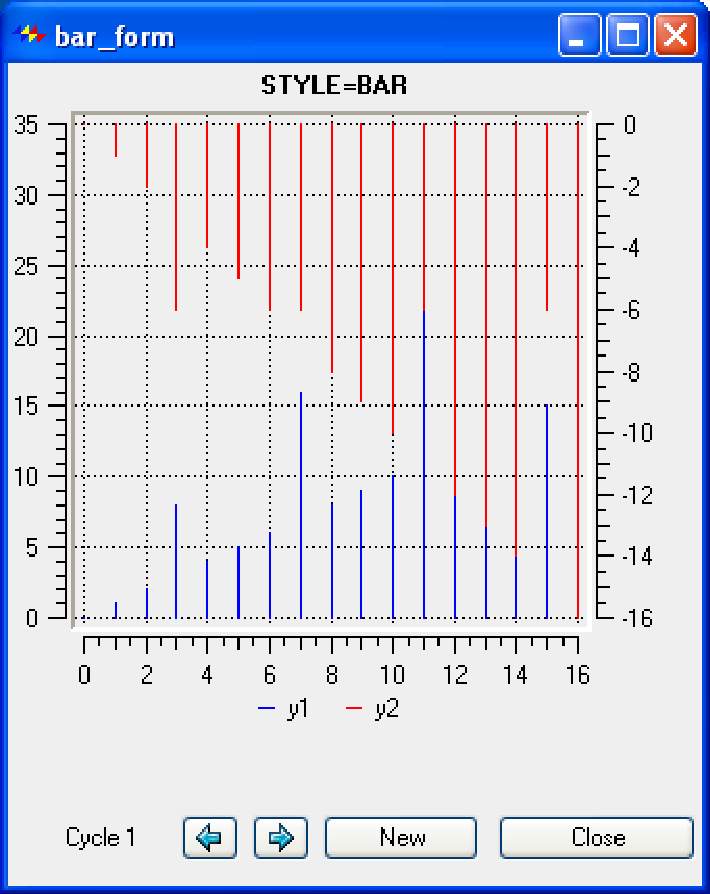
\includegraphics[width=0.8\linewidth]{plot2d-styles_bar}
        \label{hc:plot2d_style_bar}
      \end{center}
    \end{minipage}
    \hfill
    \begin{minipage}{0.45\linewidth}
      \begin{center}
        \index{PLOT2D@\PLOTTWOD!plot styles!AREA@\AREA}
        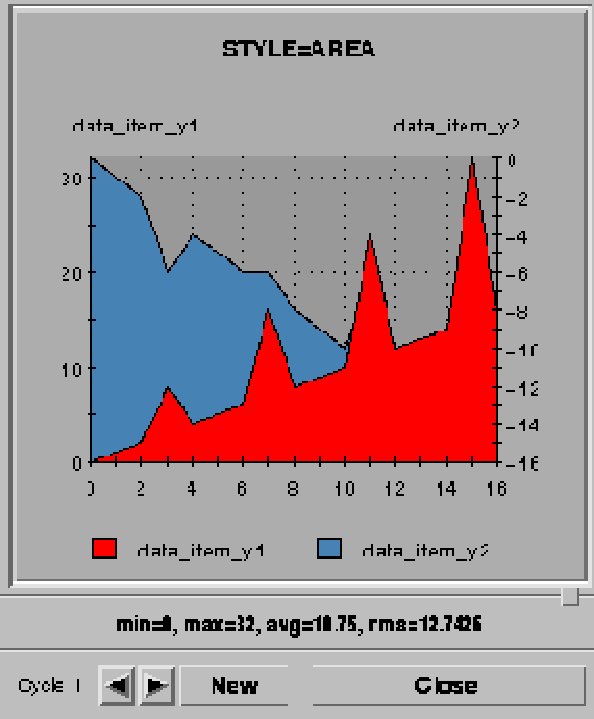
\includegraphics[width=0.8\linewidth]{plot2d-styles_area}
        \label{hc:plot2d_style_area}
      \end{center}
    \end{minipage}\\[3ex]
    %
    \begin{minipage}{0.45\linewidth}
      \begin{center}
        \index{PLOT2D@\PLOTTWOD!plot styles!PLOT@\PLOT}
        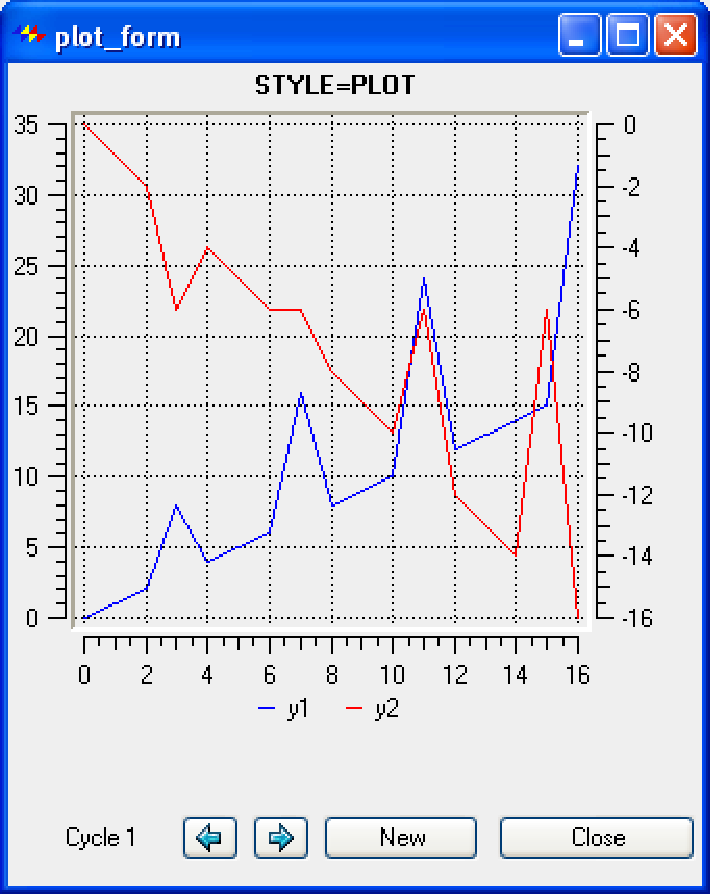
\includegraphics[width=0.8\linewidth]{plot2d-styles_plot}
        \label{hc:plot2d_style_plot}
      \end{center}
    \end{minipage}
    \hfill
    \begin{minipage}{0.45\linewidth}
      \begin{center}
        \index{PLOT2D@\PLOTTWOD!plot styles!POLAR@\POLAR}
        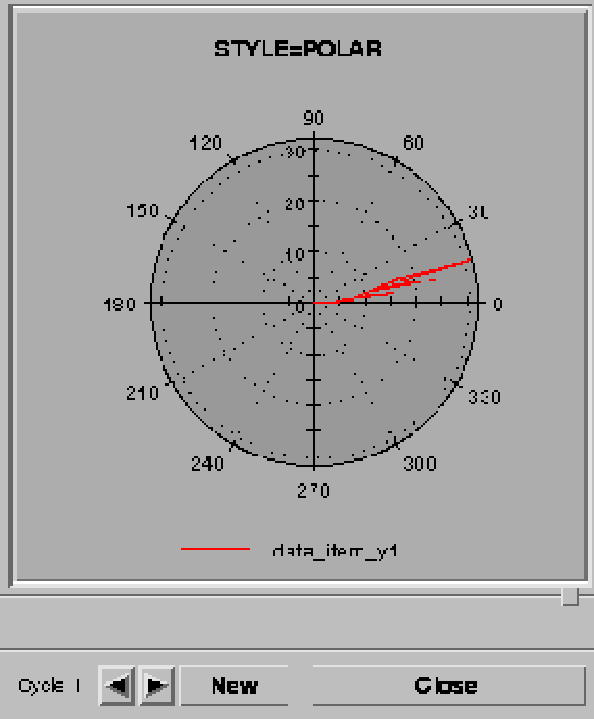
\includegraphics[width=0.8\linewidth]{plot2d-styles_polar}
        \label{hc:plot2d_style_polar}
      \end{center}
    \end{minipage}\\[3ex]
    %
    \begin{minipage}{0.45\linewidth}
      \begin{center}
        \index{PLOT2D@\PLOTTWOD!plot styles!STACKING\_BAR@\BAR}
        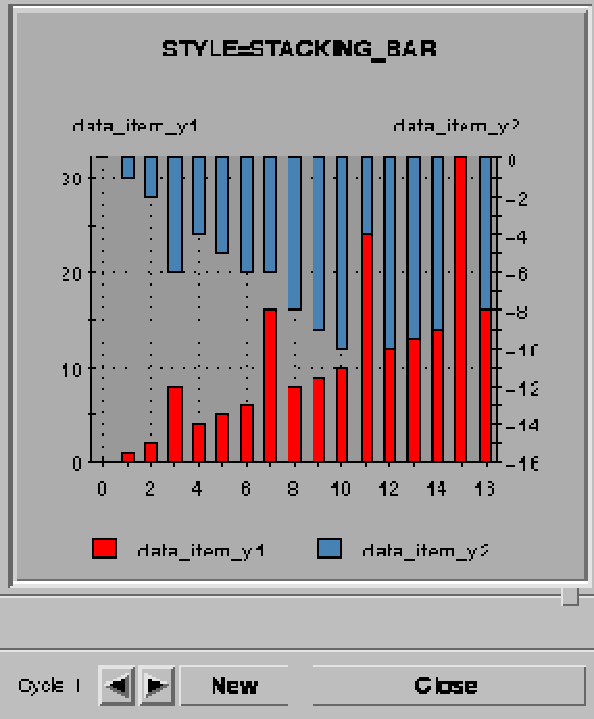
\includegraphics[width=0.8\linewidth]{plot2d-styles_stacking_bar}
        \label{hc:plot2d_style_stacking_bar}
      \end{center}
    \end{minipage}
    \hfill
    \begin{minipage}{0.45\linewidth}
      \begin{center}
        \index{PLOT2D@\PLOTTWOD!plot styles!STEP@\STEP}
        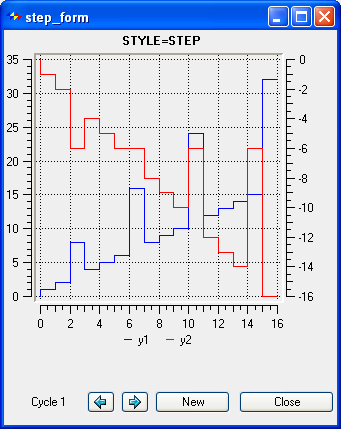
\includegraphics[width=0.8\linewidth]{plot2d-styles_step}
        \label{hc:plot2d_style_step}
      \end{center}
    \end{minipage}
  \end{center}
  \caption{Plot2d Plot styles}
\end{figure}
%
\newpage

% PLOT2D Example ASPECT_RATIO
%%%%%%%%%%%%%%%%%%%%%%%%%%%%%%%%%%%%%%%%%%%%%%%%%%%%%%%%%%%%%%%%%%%%%%%%%%%%%
\index{PLOT2D@\PLOTTWOD!example!ASPECT\_RATIO@\ASPECTRATIO}

\phantomsection
\label{des:plot2dAspectRatio}
\begin{center}
  {\LARGE Aspect Ratio \\[2ex]}
\end{center}

\begin{boxedminipage}[t]{\linewidth}
\begin{alltt}
\DESCRIPTION "PLOT2D: ASPECT_RATIO";

\DATAPOOL
  \STRUCT Axis \{
    \REAL \{\EDITABLE\}
      value
    , min \{\SCALAR\}
    , max \{\SCALAR\}
    , aspect_ratio \{\SCALAR\}
    ;
  \};
  Axis \{\SCALAR\}
    x
  , y
  ;
\END \DATAPOOL;

\UIMANAGER
  \TABLE xy_table \{
    \ORIENTATION=\VERTICAL
  , \HORIZONTAL(\TABLESIZE=15)
  \} (
    \TABLE (
      \LABEL(x)
      x.value[*]

    , \LABEL(y)
      y.value[*]
    );
  );

  \FIELDGROUP scale_fg (
    \VOID
    \LABEL(x.min)
    \LABEL(x.max)
    \LABEL(x.aspect_ratio)

  , \LABEL(x)
    x.min
    x.max
    x.aspect_ratio

  , \LABEL(y)
    y.min
    y.max
    y.aspect_ratio
  );
\end{alltt}
\end{boxedminipage}

\begin{boxedminipage}[t]{\linewidth}
\begin{alltt}
  \PLOTTWOD xy_plot (
    plot \{
      \XAXIS \{
        \LABEL=\LABEL(x)
      , \SCALE(x.min, x.max)
      , \ASPECTRATIO=x.aspect_ratio
      \}
    , \YAXISONE \{
        \LABEL=\LABEL(y)
      , \SCALE(y.min, y.max)
      , \ASPECTRATIOREFAXIS
      , \ASPECTRATIO=y.aspect_ratio
      \}
    \} (
      ( x.value[*] \{
          \XAXIS
        , LABEL=LABEL(x)
        \}
      , y.value[*] \{
          \YAXISONE
        , \LABEL=\LABEL(x)
        \}
      )
    )
  );

  \FORM main_form \{\MAIN\} (
    ( ( xy_table
      , scale_fg
      )
    , xy_plot
    )
  );
\END \UIMANAGER;
...
\END.
\end{alltt}
\end{boxedminipage}

%
\newpage

\begin{figure}[H]\label{hc:plot2dAspectRatio}
  \begin{center}
    {\LARGE Aspect Ratio \\[2ex]}
    %
    $range_x = range_y / aspect\_ratio_y = 400 / 0.8 = 500$
    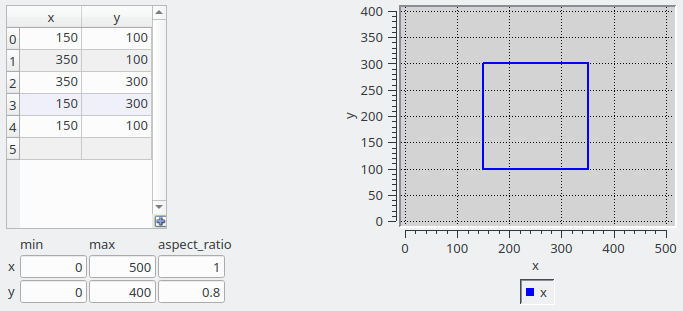
\includegraphics[width=0.8\linewidth]{plot2d-aspect_ratio-a}\\[2ex]
    %
    $ length_x = length_y / range_y * range_x * aspect\_ratio_x = length_y / aspect\_ratio_y * aspect\_ratio_x = 219 px / 0.8 * 1.5 = 411 px$
    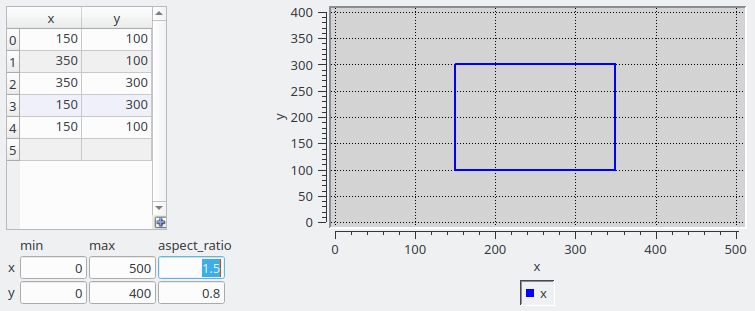
\includegraphics[width=0.8\linewidth]{plot2d-aspect_ratio-b}\\[2ex]
    %
    $range_x = range_y; length_x = length_y$
    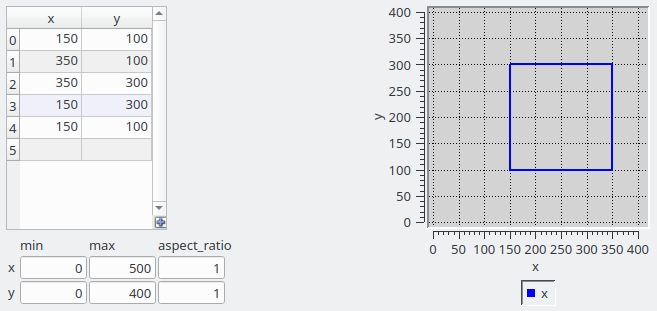
\includegraphics[width=0.8\linewidth]{plot2d-aspect_ratio-c}
  \end{center}
  \caption{Plot2d: Aspect Ratio}
\end{figure}
